\capitulo{Procedimentos metodológicos e técnicos}
\label{cap:procedimentos-metodologicos-tecnicos}

\secao{Caracterização da metodologia de pesquisa}
\label{sec:caracterizacao-metodologia-pesquisa}
    
A metodologia escolhida para o planejamento do desenvolvimento da integração entre a Amazon Alexa e o Pollen é a Metodologia em Cascata, proposta por \textcite{sommerville2011}.

A Metodologia em Cascata divide o processo em etapas sequenciais e bem definidas, garantindo que cada fase seja concluída antes de avançar para a próxima. Essa abordagem permite controle rigoroso sobre o progresso do projeto e facilita a identificação e correção de problemas durante o planejamento.

Os procedimentos técnicos adotados neste trabalho envolvem a realização de uma \textbf{pesquisa bibliográfica}, de um \textbf{estudo de caso} e o \textbf{planejamento de uma pesquisa experimental}.

A pesquisa bibliográfica fornece o embasamento teórico para definir os padrões de desenvolvimento de Alexa Skills e integração com APIs.

O estudo de caso analisa o aplicativo Pollen e identifica funcionalidades que podem ser integradas com assistentes virtuais. O enfoque é direcionado para apicultores usuários do Pollen, delimitando o escopo da pesquisa.

O planejamento da pesquisa experimental define metodologias para desenvolvimento e teste da integração Alexa+Pollen com apicultores reais, que usarão a skill em seus ambientes de trabalho. O objetivo é avaliar a eficácia da solução em contextos reais de gestão apícola.
    
    
\secao{Questões de Pesquisa}
\label{sec:questoes-pesquisa}

A integração proposta entre a Amazon Alexa e o Pollen é capaz de fornecer acesso eficiente a informações sobre colmeias através de comandos de voz, melhorando a experiência do usuário e facilitando o trabalho no apiário sem necessidade de interromper as atividades para consultar dispositivos móveis?

\secao{Aplicação da metodologia}
\label{sec:aplicacao-metodologia}

As etapas da metodologia englobam planejamento do ambiente de desenvolvimento, coleta de requisitos, implementação da integração Alexa+Pollen e validação dos resultados. Cada fase será planejada para garantir a confiabilidade do sistema e a coerência com os objetivos do trabalho.

\subsecao{Planejamento do desenvolvimento da solução proposta}
\label{ssec:planejamento-desenvolvimento-solucao}

O modelo em cascata foi originalmente descrito por Winston Royce em 1970 e estruturado por Ian Sommerville em sua obra "Engenharia de Software" como um processo sequencial onde cada fase depende da entrega da anterior.

\begin{figura}{Modelo Cascata}{\textcite{sommerville2011}}
    \begin{flushleft}
        \label{fig:modelo-cascata}
        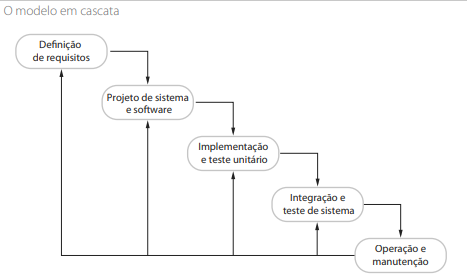
\includegraphics[width=0.95\linewidth]{resources/floats/ilustracoes/cascata.png}
    \end{flushleft}
\end{figura}

A Figura \ref{fig:modelo-cascata} ilustra as cinco fases principais do modelo: definição de requisitos, projeto de sistema e software, implementação e teste unitário, integração e teste de sistema, e operação e manutenção. Cada fase possui entregáveis específicos e critérios bem definidos.

\subsubsecao{Definição de Requisitos}
\label{sssec:def-requisitos}

A definição de requisitos descreve o que o sistema deve fazer e quais restrições deve obedecer. \textcite{sommerville2011} define requisito como "uma descrição de algo que o sistema deve fazer ou uma propriedade que ele deve ter" \cite[p. 82]{sommerville2011}. Essa definição engloba funcionalidades esperadas e limitações técnicas ou organizacionais.

Os requisitos funcionais especificam os serviços que o sistema deve oferecer e como deve reagir a entradas específicas. Os requisitos não funcionais dizem respeito a restrições sobre os serviços, como desempenho, padrões de qualidade, requisitos organizacionais ou de segurança. Para obter esses requisitos, serão realizadas entrevistas semiestruturadas com apicultores usuários do Pollen. Essa abordagem permite captar as necessidades práticas dos usuários, possibilitando uma definição mais precisa dos requisitos.

\subsubsecao{Projeto de Sistema e Software}
\label{sssec:proj-sistema}

A fase de projeto transforma os requisitos em uma arquitetura viável para implementação. \textcite{sommerville2011} define o projeto de software como o processo de definir a arquitetura, os componentes e suas interfaces, garantindo que o sistema satisfaça os requisitos especificados. Essa etapa se desdobra em três frentes: desenvolver uma Alexa Skill personalizada, integrar com o Pollen e testar a integração com usuários reais.

O desenvolvimento da Alexa Skill será feito usando o Amazon Alexa Skills Kit e Node.js, seguindo as melhores práticas. O processo envolve registro da skill no Amazon Developer Console, configuração do modelo de interação e desenvolvimento do backend usando AWS Lambda.

A integração com o Pollen será realizada através de chamadas HTTP para a API RESTful existente, usando autenticação JWT e seguindo as melhores práticas de segurança. 

Os testes serão feitos com usuários reais usando o Pollen e a Alexa Skill desenvolvida.

As Figuras \ref{fig:criacao-skill}, \ref{fig:linguagens-skill} e \ref{fig:teste-skill} ilustram as etapas do desenvolvimento no Amazon Developer Console. A Figura \ref{fig:criacao-skill} mostra a interface de criação da Skill, onde são configurados nome, idioma e informações básicas. A Figura \ref{fig:linguagens-skill} demonstra as opções de idiomas disponíveis — a Skill será desenvolvida em português brasileiro. A Figura \ref{fig:teste-skill} apresenta a interface de teste, ferramenta essencial para simular comandos de voz e verificar as respostas antes da publicação.

A skill permitirá consultas sobre número de colmeias, produção de mel, status dos enxames, próximas atividades de manejo e estatísticas de produtividade.

A implementação seguirá as melhores práticas de desenvolvimento de Alexa Skills: intents bem definidos, utterances em português brasileiro e respostas em formato SSML.

\begin{figura}{Tela de criação de Skill Alexa}{O Autor}
    \begin{flushleft}
        \label{fig:criacao-skill}
        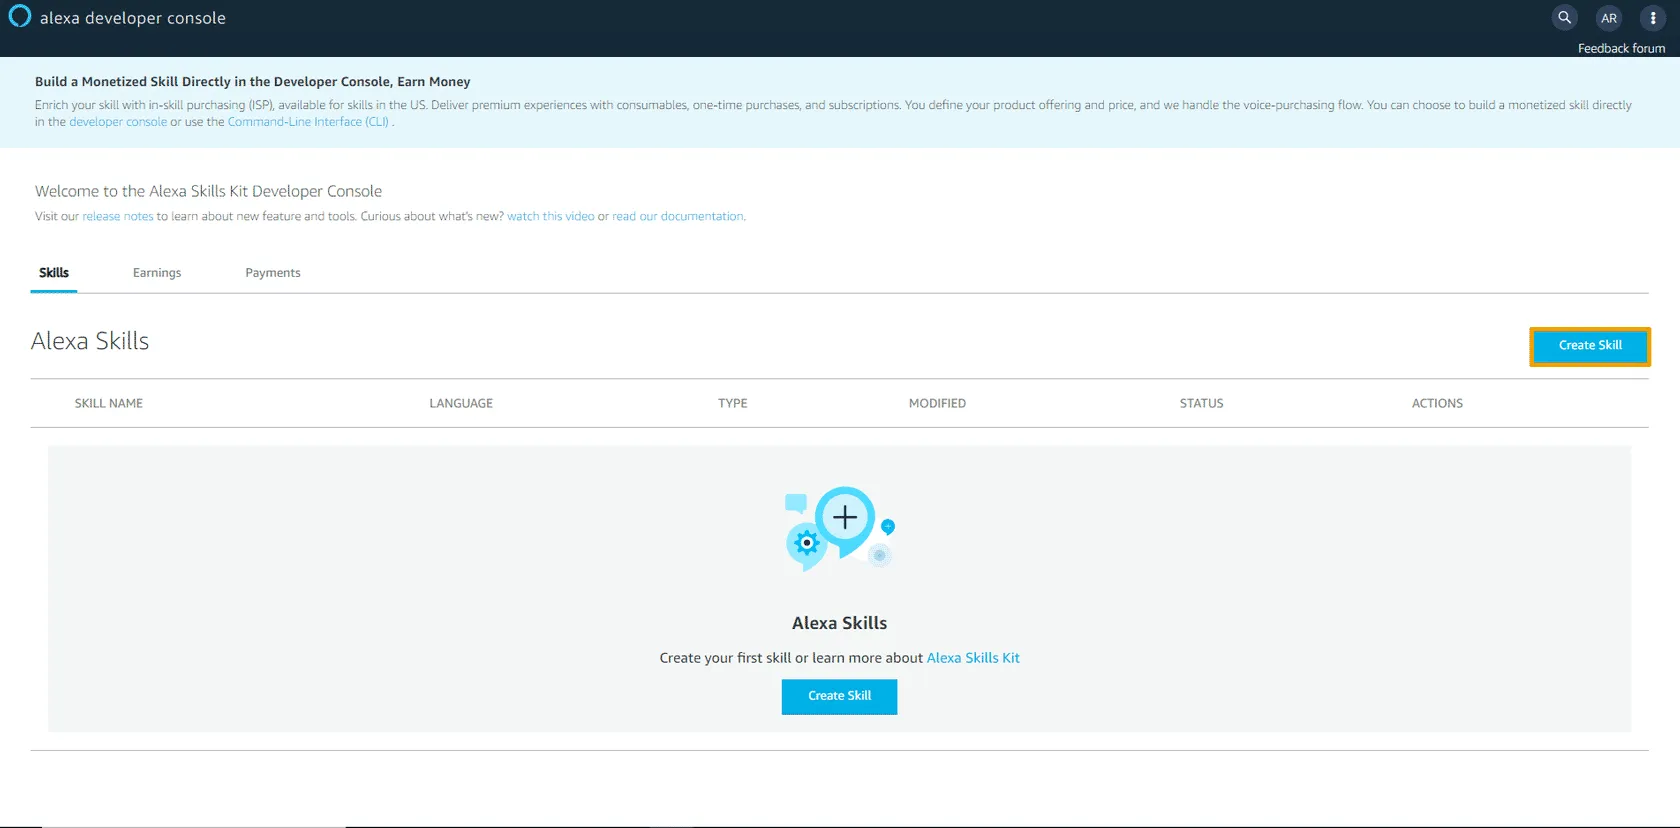
\includegraphics[width=0.85\linewidth]{resources/floats/ilustracoes/tela_criacao_skill_alexa.png}
    \end{flushleft}
\end{figura}

\begin{figura}{Tipos de linguagem aceitas pela Skill}{O Autor}
    \begin{flushleft}
        \label{fig:linguagens-skill}
        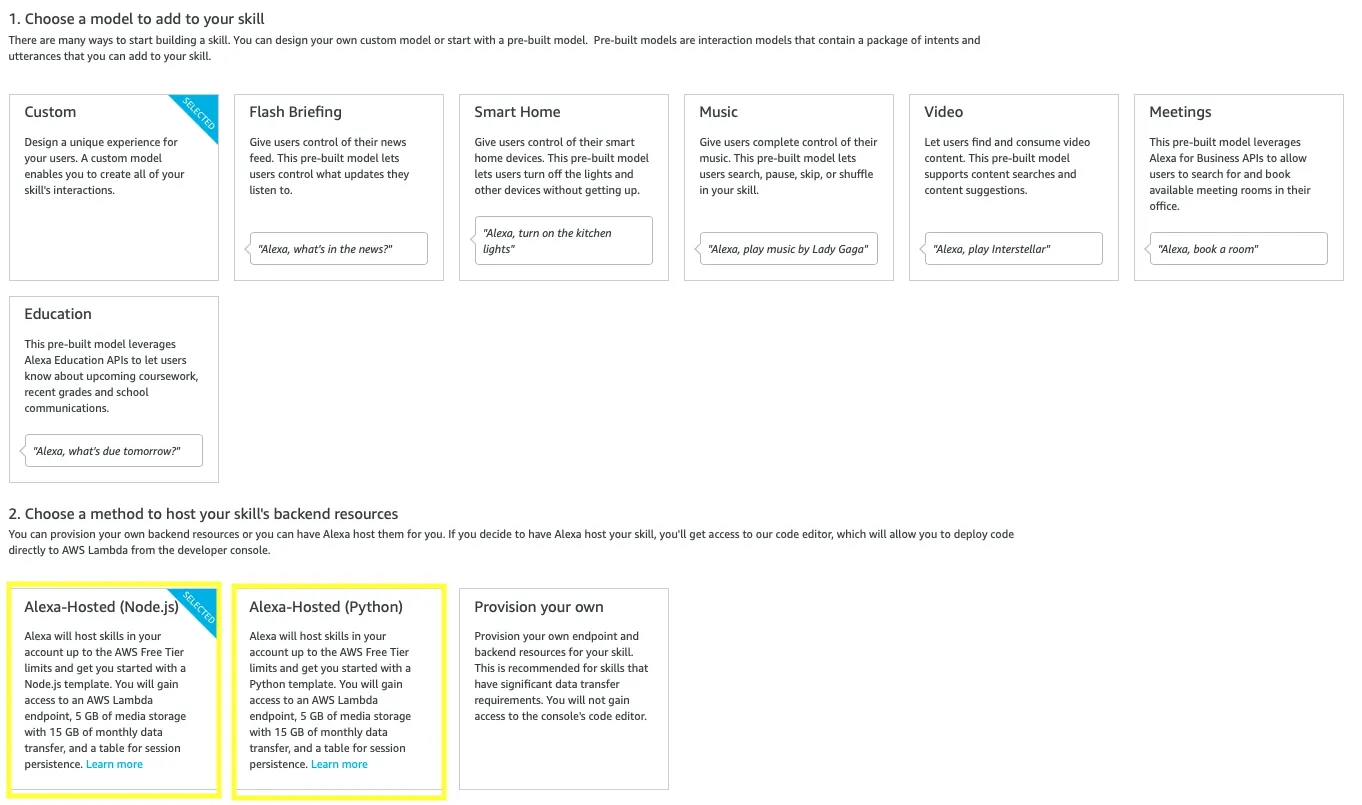
\includegraphics[width=0.85\linewidth]{resources/floats/ilustracoes/tipos_linguagem_aceitas_skill.png}
    \end{flushleft}
\end{figura}

\begin{figura}{Interface de teste da Skill Alexa}{O Autor}
    \begin{flushleft}
        \label{fig:teste-skill}
        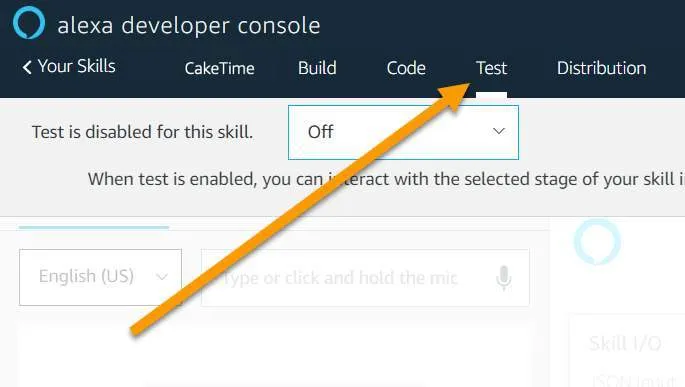
\includegraphics[width=0.85\linewidth]{resources/floats/ilustracoes/tela_para_testar_skill_criada.png}
    \end{flushleft}
\end{figura}

\subsubsecao{Fase de Implementação}
\label{sssec:implementação}

A fase de implementação concretiza as decisões de projeto na construção prática do sistema. \textcite{sommerville2011} define essa etapa como a transformação dos modelos em código executável, respeitando os padrões estabelecidos e validando o funcionamento do sistema. 

O desenvolvimento da Alexa Skill será realizado usando Node.js e o Amazon Alexa Skills Kit (ASK). A skill será hospedada como função AWS Lambda, garantindo escalabilidade e confiabilidade. A comunicação com a API do Pollen será implementada usando bibliotecas HTTP nativas do Node.js, com tratamento de erros e timeouts.

A linguagem escolhida é Node.js com TypeScript. Serão usadas as bibliotecas oficiais do Alexa Skills Kit e bibliotecas para comunicação HTTP e processamento JSON. A programação será feita na IDE VS Code, que permite integração com ferramentas de versionamento.

O repositório será controlado via Git e hospedado no GitHub, garantindo controle de versão, rastreabilidade de mudanças e backup. Isso também permitirá integração com pipelines de entrega contínua, caso a aplicação seja expandida.

\subsubsecao{Tecnologias Utilizadas}
\label{sssec:tecnologias}

O desenvolvimento usará \textbf{Node.js com TypeScript} para implementação da Skill, devido ao suporte oficial da Amazon. A Skill será hospedada em \textbf{AWS Lambda}, garantindo escalabilidade e disponibilidade. A comunicação com o Pollen ocorrerá via \textbf{API RESTful} existente, usando autenticação \textbf{JWT} e protocolo \textbf{HTTPS} para segurança. O banco de dados \textbf{PostgreSQL} do Pollen será acessado indiretamente através da API, mantendo a arquitetura de camadas.

\subsubsecao{Fase de integração e testes}
\label{sssec:testes}

A fase de testes garante a qualidade do software e a conformidade com os requisitos especificados. \textcite{pressman2011} afirma que os testes devem ser planejados de forma sistemática para revelar o maior número possível de defeitos, contribuindo para a qualidade e confiabilidade do produto final.

Os testes serão divididos entre verificação funcional da Alexa Skill e avaliação da integração com a API do Pollen. O roteiro considera a execução da skill com comandos de voz reais, testados por apicultores usuários do Pollen. O objetivo é validar se as consultas por voz funcionam corretamente, se os dados retornados atendem os critérios esperados e se a experiência de uso permanece fluida. As verificações incluem reconhecimento correto dos comandos, comunicação adequada com a API, formatação apropriada das respostas em SSML e bom desempenho geral. Parte dos testes será automatizada usando o framework Jest, focando em processamento de intents e validação da integração com a API.

Os testes incluirão: testes unitários (processamento de intents e validação de dados), testes de integração (comunicação com API Pollen) e testes de aceitação do usuário (comandos de voz reais). Os critérios de sucesso são: precisão de reconhecimento mínima de 90\%, tempo de resposta máximo de 3 segundos e satisfação do usuário de pelo menos 4.0/5.0. Os formulários de avaliação estão no Apêndice C.

\subsubsecao{Operação e manutenção}
\label{sssec:operação}

A fase de operação e manutenção é a última etapa do ciclo de vida no modelo em cascata. Ela garante a continuidade do funcionamento do sistema após a entrega e contempla ajustes, correções de falhas e melhorias que surgirem com o uso contínuo. \textcite{pressman2016} explica que esta etapa envolve a correção de erros não detectados anteriormente e a adaptação do software às mudanças de ambiente e requisitos.

Neste trabalho, serão feitas manutenções para o bom funcionamento do sistema, buscando atualizações que melhorem sua eficiência. Melhorias futuras podem incluir implementação de novos comandos de voz, integração com outros assistentes virtuais ou expansão das funcionalidades de consulta.

\subsecao{População e Amostra}
\label{sec:esboco-projeto-pratica}

A população deste estudo é composta por apicultores usuários do Pollen que possuem dispositivos Amazon Echo ou compatíveis com Alexa. O aplicativo conta com aproximadamente 150 usuários ativos, dos quais estima-se que 30\% (45 usuários) possuem ou têm acesso a dispositivos compatíveis com Alexa.

Para os testes de validação, será selecionada uma amostra de 10 a 15 apicultores usuários do Pollen que possuem dispositivos Amazon Echo ou compatíveis. A seleção seguirá os critérios:

\begin{itemize}
    \item \textbf{Disponibilidade de dispositivo}: Possuir Amazon Echo, Echo Dot ou outro dispositivo compatível com Alexa
    \item \textbf{Experiência com apicultura}: Incluir apicultores com diferentes níveis de experiência (iniciantes, intermediários e experientes)
    \item \textbf{Tamanho de operação}: Variar entre pequenos apicultores (até 10 colmeias), médios (11 a 50 colmeias) e grandes (mais de 50 colmeias)
    \item \textbf{Uso ativo do Pollen}: Usuários que utilizam o aplicativo regularmente para gestão de suas colmeias
    \item \textbf{Disponibilidade para participação}: Disposição para testar a Skill e responder aos formulários de avaliação
\end{itemize}

A amostra de 10 a 15 participantes é considerada adequada para um estudo qualitativo de validação de interface de voz, permitindo identificar problemas de usabilidade e avaliar a eficácia da solução. A seleção considerará apicultores de diferentes níveis de experiência e tamanhos de operação, permitindo avaliar a aplicabilidade da integração Alexa+Pollen em contextos reais de gestão apícola.

\secao{Coleta e Análise dos resultados da solução}
\label{sec:coleta-analise-resultados}

A coleta e análise dos resultados será realizada em três etapas: definição dos experimentos, seleção dos participantes e análise dos dados.

A primeira etapa determina quais experimentos serão realizados. Para a integração Alexa+Pollen, a avaliação incluirá testes de funcionalidade e aceitação do usuário. Os experimentos serão realizados através de formulários com escala Likert.

Dois tipos de avaliação serão utilizados: avaliação de funcionalidades do sistema (verifica se os requisitos foram cumpridos totalmente, parcialmente ou não cumpridos) e avaliação de eficácia da solução (relacionada aos critérios de sucesso e aceitação).

A segunda etapa define os participantes. Os experimentos serão realizados por apicultores usuários do Pollen que possuem dispositivos Amazon Echo ou compatíveis com Alexa. 

Para validar a necessidade e interesse dos usuários pela integração Alexa+Pollen, foi realizada uma pesquisa preliminar utilizando Google Forms, enviada por e-mail para usuários ativos do aplicativo Pollen. A pesquisa contou com 5 respondentes e apresentou os seguintes resultados:

\textbf{Resultados da Pesquisa Preliminar:}

A pesquisa "Pollen integração com ALEXA" foi aplicada para 5 usuários do aplicativo Pollen, obtendo os seguintes resultados:

\begin{itemize}
    \item \textbf{Interesse na integração}: 100\% dos respondentes (5/5) manifestaram interesse na integração do aplicativo Pollen com Alexa
    \item \textbf{Funcionalidades desejadas pelos usuários}:
    \begin{itemize}
        \item Perguntas sobre idade da rainha
        \item Consulta sobre força do enxame
        \item Data da última divisão
        \item Quantidade de enxames de determinada espécie
        \item Produção de mel de determinada espécie
        \item Notificações e rotinas (lembrete de manutenção da colmeia ou alimentação)
        \item Registro de localização do Meliponário
    \end{itemize}
    \item \textbf{Sugestões de assistentes virtuais}: Os usuários mencionaram preferência por Alexa e Google Assistant
    \item \textbf{Funcionalidades específicas sugeridas}:
    \begin{itemize}
        \item Passo a passo de cuidados com a colmeia
        \item Consulta de quantidade de enxames
        \item Registro de data das divisões
    \end{itemize}
\end{itemize}

Estes resultados validam a necessidade identificada no problema de pesquisa e demonstram que os usuários do Pollen têm interesse real na integração com assistentes virtuais, especialmente para consultas rápidas e registro de informações durante o trabalho no apiário.

A terceira etapa define como será feita a análise dos dados coletados. 

Para o formulário de avaliação de funcionalidades, a solução será considerada funcional se atingir média 7. \textcite{junek2014} justifica essa escolha:

"[...] não dá para tirar 7 sem interferência do estudo. A probabilidade de tirar um 7, sem saber nada, em uma prova de 10 questões com 4 alternativas, sendo apenas 1 delas correta, é de 0,003. Ou seja, você terá que fazer mil provas chutando os resultados para em três das mil tirar notas 7. Desta forma, se entende que um aluno que tira um 7, só pode ter sido por conta do estudo."

O cálculo da média de funcionalidade dar-se-á por meio da seguinte fórmula matemática, estabelecida por \textcite{campagnaro2017}:

\begin{equation}
\text{MédiaFunc} = \frac{(\sum \text{QtdA} + \sum \text{QtdEP} \times 0,5)}{N \times \text{QtdAva}} \times 10
\end{equation}

Onde: 
\begin{itemize}
    \item $\sum QtdA$: Somatório de alternativas marcadas como Atendidas.
    \item $\sum QtdEP$: Somatório de alternativas marcadas como Atendidas em parte.
    \item $\sum QtdEP \times 0,5$: Divide-se por 2 (dois) o $\sum QtdEP$, devido ao fato de que atendimento em parte possui à metade do peso das consideradas atendidas.
    \item $N$: É a quantidade de questões de funcionalidades avaliadas.
    \item $QtdAva$: É a quantidade de avaliadores/participantes.
    \item $\times 10$: Para se obter já a média na escala de 0 a 10.
\end{itemize}

Para o formulário de avaliação de eficácia/aceitação, a solução será considerada funcional se atingir média igual ou superior a 3,5. Esse valor foi escolhido considerando que cada opção da escala Likert possui um peso diferente, permitindo melhor captura da percepção dos avaliadores.

Os pesos de cada opção da escala são:
\begin{itemize}
    \item Concordo fortemente = 5
    \item Concordo = 4
    \item Indeciso = 3
    \item Discordo = 2
    \item Discordo fortemente = 1
\end{itemize}

A fórmula matemática que irá avaliar a eficácia é a seguinte:

\begin{equation}
\text{MédiaEfi} = \frac{(\sum \text{CF} \times 5 + \sum \text{C} \times 4 + \sum \text{I} \times 3 + \sum \text{D} \times 2 + \sum \text{DF} \times 1)}{N \times \text{QtdAva}}
\end{equation}

Onde: 
\begin{itemize}
    \item $\sum CF$: Somatório da escala concordo fortemente;
    \item $\sum C$: Somatório da escala concordo;
    \item $\sum I$: Somatório da escala indeciso;
    \item $\sum D$: Somatório da escala discordo;
    \item $\sum DF$: Somatório da escala discordo fortemente;
    \item $N$: É a quantidade de critérios de eficácia avaliados;
    \item $QtdAva$: É a quantidade de avaliadores/participantes.
\end{itemize}

A análise também pode ser realizada a partir de média simples, média ponderada, mediana e quaisquer outros métodos estatísticos, bem como pelo simples conhecimento empírico.






